\chapter{Ligaduras no holónomas}

	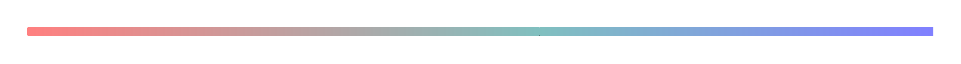
\begin{tikzpicture}
	\fill [left color=red!50, right color=teal!50] (0,0) rectangle (6.5,.1);
	\fill [left color=teal!50, right color=blue!50] (6.5,0) rectangle (11.5,.1);
	\end{tikzpicture}


\vspace{10mm}
\begin{adjustwidth}{50pt}{50pt}
\begin{ejemplo}
El problema que vamos a resolver es el del movimiento de un robot en la superficie de Marte. El robot podrá girar sobre su CM y se puede desplazar rectilíneamente sobre su eje.

Exigiremos que el robot \emph{no derrape}, que su vector velocidad sea paralela a su eje. Este será nuestro ejemplo (típico) de ligadura no holónoma.

\begin{figure}[H]
		\centering
		\includegraphics[width=.75\textwidth]{imagenes/img09-01.png}
	\end{figure}

\vspace{2mm}
\end{ejemplo}
\end{adjustwidth}

\begin{myblock}{Principio de Hamilton}

\begin{large}
\begin{equation}
\boldsymbol{
S\ = \ \displaystyle \int_{t_1}^{t_2} \ L(q_j,\ \dot q_j,\ t) \ \dd t 
\quad \quad \to \quad \quad \var S\ = \ 0
}
\end{equation}
\end{large}
\end{myblock}


\section{Ligaduras no holónomas}

Hasta ahora solo hemos visto \emph{ligaduras holónomas}, en que podemos expresar las coordenadas de las partículas en función de las coordenadas generalizadas y del tiempo, $\ \vec r=\vec r(q_i,t)\, . \ $ Cuando esto no es posible, decimos que las ligaduras son \emph{\textbf{no holónomas}}.

Por motivos de claridad en la exposición, consideraremos que solo tenemos dos coordenadas generalizadas, $\ q_1 \text{ y } q_2$ (la extensión a mayor número de variables generalizadas es trivial).

En las ligaduras \emph{no holónomas} se imponen condiciones del tipo:

\begin{equation}
\label{T9Def1LNH}
\mqty(\xmat*{a}{2}{2}) \ \mqty(\dot q_1 \\ \dot q_2)  \ = \ - \mqty(a_{10}\\a_{20})
\end{equation}

\textcolor{gris}{(encontraremos sentido a este modo de imponer ligaduras cuando abordemos el problema del robot en Marte).}

De otro modo, $\qquad  \displaystyle \ \mqty(\xmat*{a}{2}{2}) \ \mqty(\dv{t} q_1 \\ \dv{t} q_2)  \ = \ - \mqty(a_{10}\\a_{20})\, , \ $ despejando

\begin{equation}
\label{T9LNH}
\mqty(\xmat*{a}{2}{2}) \ \mqty(\dd q_1 \\ \dd q_2)  \ = \ - \mqty(a_{10}\\a_{20}) \ \dd t
\end{equation}

Ambas maneras de expresar las ligaduras no holónomas son equivalentes.

Recordemos que un \emph{desplazamiento virtual} ocurre cuando el tiempo está fijo (congelado):  $\qquad $  $\qquad $ $\boldsymbol{\var q \ = \ {(\dd q)}_{\, t\ fijo}}\, , \ $ (ver sección \ref{T1PTV}). Pues bien, para desplazamientos virtuales, si el tiempo es fijo, en la definición de ligaduras no holónomas de las ecuaciones \ref{T9LNH}, $\ \dd t=0 \to $

$\displaystyle  \to \ \mqty(\xmat*{a}{2}{2}) \  \mqty(\var   q_1 \\ \var   q_2) \ = \ M  \  \mqty(\var  q_1 \\ \var  q_2) \ = \  \mqty(0 \\ 0) \, . \ $ 

Si $|M|=0$, tendremos un sistema compatible determinado que, como es homogéneo, tendrá solución única: la trivial, $\var q_1 = \var q_2=0$. No hay movimiento posible en el sistema. Esto es una contradicción, por lo que $|M| \neq 0$, con lo que las filas de la matriz $M$ serán proporcionales, $(a_{11} \ a_{12}) = k (a_{21} \ a_{22})$. Solo quedará una ecuación libre: $\boldsymbol{ \  a_{11} \ \var q_1 \ + \   a_{12} \ \var q_2 \ = \  0\, , \  }$ en el caso 2D (2 coordenadas generalizadas). 

\emph{``Para ligaduras holónomas las variables generalizadas son independientes, en las no holónomas hay relaciones entre ellas''.}

Del principio de Hamilton cuando las ligaduras son holónomas se obtienen las ecuaciones de Euler-Lagrange, $\ \displaystyle \pdv{L}{q_j} - \dv{t} \left( \pdv{L}{\dot q_j} \right)  = 0$. Veamos que ocurre con las ligaduras no holónomas.

$$ \displaystyle \var S = \int_{t_1}^{t_2} \ \left\{ \ \ 
\left[ \pdv{L}{q_1} - \dv{t} \left( \pdv{L}{\dot q_1} \right) \right] \ \var q_1 \ + \ 
\left[ \pdv{L}{q_2} - \dv{t}  \left( \pdv{L}{\dot q_2} \right) \right] \ \var q_2
 \ \right\} \ = \ 0 $$
 
 Como ahora (ligaduras no holónomas) $\var q_1 \text{ y } \var q_2$ no son independientes, no podemos exigir que ambos integrandos sean cero. Despejando de la ecuación libre que relacionaba ambas variables, $\ a_{11} \ \var q_1 \ + \   a_{12} \ \var q_2 \ = \  0 \ \to \ \var q_2 \ = \ -\dfrac {a_{11}}{a_{12}} \ \var q_1 \, , \ $ por lo que
 
 
$\displaystyle \left[ \pdv{L}{q_1} - \dv{t} \left( \pdv{L}{\dot q_1} \right) \right] \ \var q_1 \ - \ 
\left[ \pdv{L}{q_2} - \dv{t} \left( \pdv{L}{\dot q_2} \right) \right] \ \dfrac {a_{11}}{a_{12}} \ \var q_1 \ = \ 0 $

$\displaystyle \left[ \ 
\left[ \pdv{L}{q_1} - \dv{t} \left( \pdv{L}{\dot q_1} \right) \right] \ - \ 
\left[ \pdv{L}{q_2} - \dv{t} \left( \pdv{L}{\dot q_2} \right) \right] \ \dfrac {a_{11}}{a_{12}} \ \right] \ 
 \cancelto{\neq 0}{\var q_1} \ = \ 0  \ \to$
 
 $\displaystyle \ \to \ 
 \left[ \ 
\left[ \pdv{L}{q_1} - \dv{t} \left( \pdv{L}{\dot q_1} \right) \right] \ - \ 
\left[ \pdv{L}{q_2} - \dv{t} \left( \pdv{L}{\dot q_2} \right) \right] \ \dfrac {a_{11}}{a_{12}} \ \right] \ = \ 0$

$$\boldsymbol{
\displaystyle \left[ \pdv{L}{q_1} - \dv{t} \left( \pdv{L}{\dot q_1} \right) \right] \ a_{12} \ = \ 
\left[ \pdv{L}{q_2} - \dv{t} \left( \pdv{L}{\dot q_2} \right) \ \right] \ a_{11}  }$$

Que son las \textbf{ecuaciones de Euler-Lagrange modificadas para el caso de ligaduras no holónomas}.

Para escribir esto más elegantemente vamos a usar el \emph{truco} que se le ocurrió a Lagrange:

\vspace{5mm}
\subsection{Multiplicadores de \emph{Lagrange}}
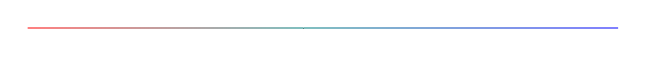
\begin{tikzpicture}
	\fill [left color=red!50, right color=teal!50] (0,0) rectangle (3.5,.01);
	\fill [left color=teal!50, right color=blue!50] (3.5,0) rectangle (7.5,.01);
	\end{tikzpicture}
\vspace{0.5cm}

Dividiendo la expresión anterior entre $\ a_{11} \ a_{12}\, ,$

$\dfrac{\displaystyle  \left[ \pdv{L}{q_1} - \dv{t} \left( \pdv{L}{\dot q_1} \right) \right]}{a_{11}} \ = \ \dfrac{\displaystyle  \left[ \pdv{L}{q_2} - \dv{t} \left( \pdv{L}{\dot q_2} \right) \ \right]}{a_{12}} \ = \ \boldsymbol{- \lambda}$ \hspace{1cm}\textcolor{gris}{(truco)}

$\displaystyle \pdv{L}{q_1} - \dv{t} \left( \pdv{L}{\dot q_1} \right)  \ = \ -\lambda \ a_{11} 
\qquad \text{ y } \qquad
\pdv{L}{q_2} - \dv{t} \left( \pdv{L}{\dot q_2} \right)  \ = \ -\lambda \ a_{12} $

Multiplicando por $- 1$,

\begin{equation}
	\subrayado{\boxed{ \ \boldsymbol{ 
	\dv{t}\left( \pdv{L}{\dot q_1} \right) - \pdv{L}{q_1}  = \lambda a_{11}
	} \ }}
	\qquad \qquad 
	\subrayado{\boxed{ \ \boldsymbol{ 
	\dv{t}\left( \pdv{L}{\dot q_2} \right) - \pdv{L}{q_2}  = \lambda a_{12}
	} \ }}
\end{equation}
\begin{center} Ecuaciones de Euler-Lagrange para el caso 2D de ligaduras no holónomas. \end{center}

\vspace{1cm}
\begin{myalertblock}{En general}

Ligaduras no holónomas: $\quad \displaystyle \boldsymbol{
\sum_{j=1}^n a_{ij} \dot q_j = -a_{i_0}\, ;\ 
\qquad  
\sum_{j=1}^n a_{ij} \dd q_j = -a_{i0} \dd t \, ;\ 
 }	 \quad i=1,2, \cdots , p$
 
\vspace{5mm} Ecuaciones Euler-Lagrange para ligaduras no holónomas:

\begin{large}
$$\displaystyle \subrayado{ \ \boxed{ \ \boldsymbol{
\dv{t}\left( \pdv{L}{\dot q_j} \right) - \pdv{L}{q_j}  = \sum_{i=1}^p \lambda_i a_{ij}
} \ } \ }$$
\end{large}
 
\end{myalertblock}




\vspace{1cm}
\subsection{Aplicación: problema del robot en Marte}
\label{T4SecELF}
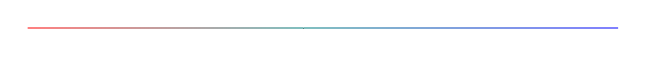
\begin{tikzpicture}
	\fill [left color=red!50, right color=teal!50] (0,0) rectangle (3.5,.01);
	\fill [left color=teal!50, right color=blue!50] (3.5,0) rectangle (7.5,.01);
	\end{tikzpicture}
\vspace{0.5cm}

\begin{example}

\begin{multicols}{2}
\begin{figure}[H]
		\centering
		\includegraphics[width=.45\textwidth]{imagenes/img09-02.png}
	\end{figure}	
	
	El robot puede girar sobre su CM y desplazarse según su eje pero sin derrapar (ligadura no holónoma): la velocidad del centro de masas del robot ha de ser paralela a su eje.

\vspace{2mm} Con $\overrightarrow R \text{ y } \theta$ tenemos determinada la posición del robot. 

\vspace{2mm} Si no hubiese ninguna restricción, el lagrangiano del sistema sería (como en la sección \ref{T5ELroracion}).

\begin{equation}
\tag{\ref{T5Lconrotacion}}
L \ = \ \dfrac{M}{2}\ \ V_{CM}^2 \ + \ \dfrac 1 2 \ I_{CM}\  \ \dot \theta^2	
\end{equation}
\end{multicols}

\vspace{2mm} Como $\overrightarrow R(x,y);\ \overrightarrow V(x,y) \ \to \ L=\dfrac M 2 (\dot x^2 + \dot y^2)+\dfrac{I_{cm}}{2} \dot \theta^2$


\vspace{5mm}Imponemos ahora la restricción de la ligadura no holónoma de que el robot no pueda derrapar: $\ \overrightarrow V_{CM} \ || \ $ eje del robot.

\vspace{2mm}$\overrightarrow V=(V_x,V_y)=(V\cos \theta,\, V\sin \theta) \ \to \ \tan \theta=\dfrac {V_y} {V_x} \ \to V_x \tan \theta = V_y \ \to \ V_x \dfrac{\sin \theta}{\cos \theta}=V_y  \to \ V_x\sin \theta  = V_y \cos \theta \ \to \quad  \sin \theta \ \dot x = \cos 	\theta \ \dot y$

\vspace{2mm} En nuestro caso, las variables generalizadas son: $\ q_1=x;\ q_2=y;\ q_3=\theta$

\vspace{2mm}
\begin{equation}
\label{T9EjLNH}
\text{Ligadura no holónoma: } \qquad \boxed{\bold{ \ \sin \theta \ \dot x = \cos 	\theta \ \dot y \ }}
\qquad \qquad \textcolor{gris}{(\sin \theta \ \dot q_1 = \cos 	\theta \ \dot q_2)}
\end{equation}

\vspace{2mm} Identificando con el caso general


\vspace{2mm}
Asimilando esto a la definición de ligaduras no holónomas, ec. \ref{T9Def1LNH}, podemos escribir:

\vspace{2mm} 
$\mqty(\sin \theta & -\cos \theta & 0 \\ 0&0&0 \\ 0&0&0  ) \ \mqty(\dot q_1 \\ \dot q_2 \\ \dot q_3) \ = \ \mqty(0\\0\\0) \qquad $
Identificamos: $\ \  \boldsymbol{a_{11}=\sin \theta\,;\ \ a_{12}=\cos \theta}$

\vspace{2mm} Escribamos las ecuaciones de Euler-Lagrange para el caso de ligaduras no holónomas y para nuestras tres coordenadas generalizadas, $x,\ y,\ \theta$

\vspace{5mm}

Coordenada $\ \boxed{  x  }\,: \quad  \qquad  \displaystyle \dv{t} \left( \pdv{L}{\dot x} \right) - \pdv{L}{x} = \lambda \sin \theta \ \to \ \dv{t} (M\dot x) - 0 = \lambda \sin \theta$

Coordenada $\ \boxed{  y  }\,: \quad  \qquad  \displaystyle \dv{t} \left( \pdv{L}{\dot y} \right) - \pdv{L}{y} = -\lambda \cos \theta \ \to \ \dv{t} (M\dot y) - 0 = -\lambda \cos \theta$

Coordenada $\ \boxed{  \theta  }\,: \quad  \qquad  \displaystyle \dv{t} \left( \pdv{L}{\dot \theta} \right) - \pdv{L}{\theta} = 0 \ \to \ \dv{t} (I_{CM} \dot \theta) \ - \ 0 \  = 0 \ \to \ I_{CM} \ddot \theta =0$

\vspace{2mm}
\begin{equation}
	\label{T9EjEcMov}
	\boldsymbol{
	\begin{cases} 
		\ \ M \ \ddot x \ = \ \  \lambda \ \sin \theta \\
		\ \  M \ \ddot y \ = \ - \lambda \ \cos \theta \\
		\ \ \dot \theta \ = \  \omega  \ \textcolor{gris}{ = \  cte}
	\end{cases} 
	}
\end{equation}


\vspace{2mm} Integrando las ecuaciones diferenciales de movimiento,
$\quad \boxed{ \boldsymbol{\theta=\omega t + \varphi_0} \ }$

\vspace{2mm}Las ecuaciones en $\dot x \text{ y } \dot{y} $ están \emph{acopladas}, pero de la relación de ligadura, ec \ref{T9EjLNH},

\vspace{2mm}$\boldsymbol{\sin \theta \ \dot x = \cos 	\theta \ \dot y}  \ \ \to \ \begin{cases}
 \ \ddot x = \ \dfrac \lambda M \sin \theta	\ \to \ \ \sin \theta = \ \ \dfrac M \lambda \ddot x\\  \\ 
 \ \ddot y = - \dfrac \lambda M \cos \theta \ \to \ \cos \theta = \ - \dfrac M \lambda \ddot y 
 \end{cases}
 \ \to \quad  \boldsymbol{\dfrac M \lambda \ddot x \ \dot x +  \dfrac M \lambda \ddot y \ \dot y =0}$

\vspace{2mm}Simplificando, $\ \ddot x \ \dot x+\ddot y \ \dot y=0$

\vspace{2mm}Como $\displaystyle \dv{t}( \Box ^2) = 2 \ \Box \ \dot{\Box} \ \to \ 
\dv{t}( \dot{\Box}^2 )  =2 \ \dot{\Box} \ \ddot{\Box}$

\vspace{2mm}Luego, $\ 2 \ \ddot x \ \dot x+ 2 \ \ddot y \ \dot y=0 \ \to \ \displaystyle
\dv{t} (\dot x^2) + \dv{t} (\dot y^2) =0 \ \to \ 
\dv{t} (\dot x^2+\dot y^2)=0 \ \to \ 
\boldsymbol{\dot x^2+\dot y^2 = A^2} \ \textcolor{gris}{(=cte)}$
 

\vspace{2mm} Despejando de $\ \sin \theta \ \dot x = \cos 	\theta \ \dot y \ \to \ \dot y=\dfrac{\sin \theta}{\cos \theta} \ \dot x\, $ [ecuación $(^*)$] y sustituyendo en la ecuación que acabamos de encontrar: 

\vspace{2mm} $\dot x^2+\dot y^2 = A^2 \ \to \ \dot x^2+\left( \dfrac{\sin \theta}{\cos \theta} \ \dot x \right)^2 = A^2 \ \to \ 
 x^2 \ \left( 1+ \dfrac{\sin^2 \theta}{\cos^2 \theta} \right) = A^2  \ \to \ \dot x^2 \ \dfrac{1}{\cos^2 \theta} =A^2 $
 
\vspace{2mm} $\dot x^2 = A^2 \ \cos^2 \theta \ \to \ x= A \ \cos \theta\, ,\  $ tercera ecuación de movimiento, $\ \dot x=A\ \cos(\omega t+\varphi_0)$

\vspace{2mm} Integrando, $\quad \boxed{ \ \boldsymbol{x=\dfrac A \omega \ \sin(\omega t + \varphi_0) + B } \ }$

\vspace{2mm} Sustituyendo en [ecuación $(^*)$] $\quad \dot y=\dfrac{\sin \theta}{\cos \theta} \ \left( \dfrac A \omega \ \sin(\omega t + \varphi_0) + B  \right)' = A\ \sin(\omega t + \varphi_0)$

\vspace{2mm} Integrando, $\quad \boxed{ \ \boldsymbol{y=-\dfrac A \omega \ \cos(\omega t + \varphi_0) + C } \ }$


\vspace{2mm} Las ecuaciones (integradas) de movimiento son:

\vspace{2mm} \begin{equation}
 \label{T9EjEcMovoInteg}	
 \subrayado{
 \boxed{ \ \boldsymbol{x=\dfrac A \omega \ \sin(\omega t + \varphi_0) + B } \ }
 \qquad
  \boxed{ \ \boldsymbol{y=-\dfrac A \omega \ \cos(\omega t + \varphi_0) + C } \ }
  \qquad
  \boxed{ \boldsymbol{\theta=\omega t + \varphi_0} \ }
  }
 \end{equation}


\vspace{2mm} También se podría calcular el valor de $\boldsymbol \lambda$, a partir de la expresión $M\ddot x= \lambda \sin \theta \text{ ó } M\ddot y= -\lambda \cos \theta$, pero puede ser fijado con las constantes $A, \ B, \ C,\ \varphi_0$ en las condiciones iniciales del problema.

\vspace{5mm} 
\begin{multicols}{2}
\underline{Sorpresa}: Las ecuaciones $ x=\dfrac A \omega \ \sin(\omega t + \varphi_0) + B  \ \text{ e } \ 
 y=-\dfrac A \omega \ \cos(\omega t + \varphi_0) + C$ son las ecuaciones paramétricas de una \emph{circunferencia} de centro $(B,C)$ y radio $\dfrac A \omega$. Nuestro robot en la superficie de Marte, sometido a la ligadura de no derrape, estaría describiendo circunferencias indefinidamente hasta que se le acabaran las baterías. Par poseer una determinada velocidad lineal necesitaríamos que hubiese aparecido un término lineal como
 $ x=\dfrac A \omega \ \sin(\omega t + \varphi_0) + B  + \alpha t \ \text{ e } \ 
 y=-\dfrac A \omega \ \cos(\omega t + \varphi_0) + C + \beta t$, pero no ha sido así.
\begin{figure}[H]
		\centering
		\includegraphics[width=.4\textwidth]{imagenes/img09-03.png}
	\end{figure}
\end{multicols}
\end{example}

\vspace{1cm}
\begin{center}
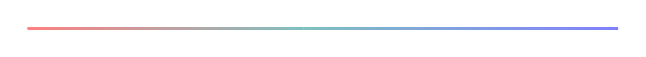
\begin{tikzpicture}
	\fill [left color=red!50, right color=teal!50] (0,0) rectangle (3.5,.02);
	\fill [left color=teal!50, right color=blue!50] (3.5,0) rectangle (7.5,.02);
	\end{tikzpicture}
\end{center}
\vspace{1cm}

\begin{myexampleblock}{Ligaduras}

\vspace{2mm} Las restricciones al movimiento en sistemas mecánicos reciben el nombre de \emph{ligaduras o vínculos}. Hay varias formas de clasificar las ligaduras. En Mecánica Teórica, la distinción más importante es entre ligaduras holónomas y no holónomas.

\vspace{2mm}  \textbf{Tipos de ligaduras}:

\vspace{2mm} Los dos criterios principales son si las ligaduras son integrables (permiten reducir el número de grados de libertad) o no y si contienen explícitamente al tiempo o no. Una ligadura no lineal se representa generalmente como una relación entre las coordenadas generalizadas necesarias para describir un sistema así como sus derivadas. Así una ligadura es cualquier expresión del tipo: $\ \Phi(q_i,\dot q_i, \ddot q_i,\cdots ,t)=0$

\begin{adjustwidth}{20pt}{5pt}
\vspace{2mm} $\triangleright \ $ Respecto a la integrabilidad de las ligaduras los sistemas se clasifican en:

\begin{adjustwidth}{20pt}{5pt}
\vspace{2mm} --- \emph{Ligaduras holónomas}. Si la expresión anterior es constante respecto a las derivadas la coordenada se llama holónoma. En ese caso las ligaduras pueden escribirse de la forma $f_j(\vec r_1, \vec r_2, \cdots \vec r_i, t)=0$. Nótese que el número $\ j \ $  condiciona al número de coordenadas que pueden existir, por lo que suele decirse que éstas ligaduras permiten eliminar grados de libertad al sistema.

\vspace{2mm} --- Ligaduras no holónomas. Cuando las coordenadas no pueden escribirse como holónomas. Así las ligaduras no holónomas no permiten eliminar los grados de libertad de un sistema. Estas ligaduras pueden clasificarse adicionalmente en lineales y no lineales.
\end{adjustwidth}

\vspace{2mm} $\triangleright \ $ Respecto a si las expresiones matemáticas que contienen las ligaduras contienen o no la variable tiempo las ligaduras se clasifican en:

\begin{adjustwidth}{20pt}{5pt}
\vspace{2mm} --- Ligaduras esclerónomas cuando las ligaduras son independientes del tiempo.

\vspace{2mm} --- Ligaduras reónomas cuando contienen al tiempo explícitamente, o sea son dependientes del tiempo.
\end{adjustwidth}
\end{adjustwidth}


\vspace{2mm} Algunos ejemplos de ligaduras son:

\begin{adjustwidth}{20pt}{5pt}
\vspace{2mm} --- Partícula moviéndose sobre una curva plana conocida $y = f(x)$, esta ligadura es holónoma.

\vspace{2mm} --- Rodamiento sin deslizamiento (ligadura lineal no holónoma), una rueda orientable de radio $R$ apoya sobre un plano sin deslizar.
\end{adjustwidth}
\vspace{2mm} 
	
\end{myexampleblock}
